\chapter{Planning Clásico}
\label{ch:lit_planning}

En este capítulo se detallan las definiciones teóricas, necesarias para
comprender el enfoque de esta tesis y sobre qué parte de este campo aplicaremos
técnicas de aprendizaje automático. Partiendo desde el área de \emph{planning},
detallando más concretamente que son los estados y acciones, representación
STRIPS de un problema, el lenguaje PDDL, el proceso de \emph{grounding}, la
complejidad de encontrar un plan que resuelva la tarea, y la necesidad de tomar
ventaja de planes relajados. Gran parte del material de este capítulo fue basado
en el trabajo ``Learning How to Ground a Plan`` llevado a cabo en
\citep{Gnad_Torralba_Dominguez_Areces_Bustos_2019}, el libro ``Planning Theory
\& Practice`` \citep{Nau-Ghallab-Malik-Traverso-2004}, y los artículos con el
funcionamiento de Fast Downward y PDDL en \citep{Helmert-2011, McDermott1998}.
Así mismo, se hizo referencia a detalles más específicos provenientes de otros
artículos científicos que también fueron de gran importancia para comprender los
fundamentos de planning clásico.

\section{¿Qué se entiende por planning?}

Durante nuestras actividades de la vida cotidiana, siempre estamos actuando y
anticipando el resultado de nuestras decisiones, aun de manera inconsciente, sin
estar explícitamente planeando que hacer antes de realizar una acción. Por otro
lado, una tarea que abarque objetivos nuevos y complejos necesita de ser
planeada conscientemente al consistir de acciones que uno no está acostumbrado,
tareas de alto riesgo, o cooperación con alguien más. Hay otras tareas en las
que incluso no pueden ser planeadas por una persona, sino que se deben
determinar de manera automática, tal es el caso por ejemplo de una operación de
rescate después de algún desastre natural, como un terremoto o inundación. La
operación podría necesitar de una gran cantidad de rescatistas, sistemas de
comunicación con una base general, y actividades de logística. Todos dependiendo
de una planificación cuidadosa y evaluación de varias alternativas en un tiempo
de rescate limitado y por ende una urgencia inmediata de toma de decisión. Este
tipo de tareas justifican el uso de herramientas de planificación automática y
son la principal motivación de \emph{Automated Planning}.

Automated Planning es el área de la inteligencia artificial que busca
automatizar tareas de planificación, en particular, tareas que resulta inviable
ser planificadas por un humano, ya sea, por razones de costos, riesgos, o
recursos. Esto se logra basándose en el razonamiento sobre representaciones
abstractas y formales del dominio, configuración inicial, combinación de
acciones, y objetivos a ser cumplidos. El modelo conceptual del dominio en el
cual las acciones son ejecutadas es llamado \emph{dominio de planning}, y los
requerimientos inicial y final son denominados \emph{estado inicial} y
\emph{meta}. Estas 3 componentes definen una \emph{tarea de planning} cuyo
objetivo es encontrar alguna combinación de acciones que determinen un
\emph{plan}.

\section{Estados y acciones}

Un estado posible de una tarea de \emph{planning} se representa a partir de un
conjunto de símbolos proposicionales que modelan aspectos del entorno. Por
ejemplo, el símbolo proposicional $p$ puede modelar la situación ``el agente
$a_1$ se encuentra en la ubicación $l_1$``. Aquellos símbolos que no están
mencionados en un estado, se asumen como falsos en dicho mundo. De esta manera,
si se tienen los símbolos proposicionales $p,q,r$, $\{p, q\}$ representa el
estado en el que $p$ y $q$ son verdaderos, pero no $r$.

Las acciones son representadas en términos de una precondición y un efecto. La
precondición es una fórmula proposicional que representa la condición necesaria
para que la acción pueda ser llevada a cabo. Mientras que el efecto es una
fórmula que determina los cambios que produce la ejecución de la acción sobre el
entorno. Por ejemplo, consideremos la siguiente acción $A$:
\begin{align*}
    & Action : A \\
    & pre : p \land \neg r \\
    & \mathit{eff} : \neg p \land q
\end{align*}

$A$ no es aplicable en el estado $\{p, r\}$, ya que, no se cumple su
precondición, pero si en el estado $\{p\}$ transformándolo en el estado $\{q\}$.
Se puede interpretar las acciones como operadores de transformación de estados
en el que su ejecución genera que ciertos símbolos proposicionales se hagan
verdaderos o falsos según si estos ocurren positivamente o negativamente en el
efecto de la acción.

El tipo de fórmula que se permite en la precondición y en el efecto de las
acciones determina el tipo de la tarea de \emph{planning}. En particular, se
utilizaron tareas de \emph{planning} STRIPS durante el desarrollo de esta tesis.

\section{Tareas STRIPS}

El tipo de una tarea de \emph{planning} está dada por la lógica de las fórmulas
que ocurren en las acciones y en la meta. En STRIPS, las fórmulas son
conjunciones de literales, es decir, son de la forma $\bigwedge_i l_i$ con $l_i$
un símbolo proposicional o su negación.

\begin{mydef}
    Una fórmula STRIPS es una fórmula $\phi$ tal que $\phi$ es de la forma
    $\bigwedge_i l_i$ con $l_i$ un literal. Una acción $a$ es del tipo STRIPS si
    su precondición y su efecto son fórmulas STRIPS.
\end{mydef}

Una forma más conveniente de trabajar sobre esta representación es utilizando
únicamente conjuntos de símbolos proposicionales. Vimos que en el caso de los
estados, solo se mantienen aquellos que son verdaderos, es decir, los literales
positivos. De manera similar, ocurre con la precondición de una acción. Sin
embargo, en el caso de su efecto se mantienen dos conjuntos, uno con los
símbolos proposicionales positivos, y otro con los negativos.

Por ejemplo, la acción $A$ que describimos anteriormente puede verse de la
siguiente forma:
\begin{align*}
    & Action : A \\
    & pre : \{ p \}\\
    & add : \{ q \}\\
    & del : \{ p \}
\end{align*}

La interpretación de $A$ es similar a la que se dio anteriormente, la
precondición contiene los símbolos proposicionales necesarios para que $A$ sea
aplicable en un estado. Mientras que $add$ y $del$ son los conjuntos de símbolos
proposicionales que agrega y elimina la acción producto de su ejecución.

Esta nueva representación permite abstraer fórmulas y operadores
proposicionales, lo cual ayudará para introducir de manera más natural algunas
técnicas del área.

Algo importante a recalcar es el orden en que se ejecuta una acción. Para un
estado aplicable de $A$ optaremos por primero eliminar los símbolos que sean
verdaderos a partir de su lista $del$ para luego agregar los de la lista $add$.
Esto con el fin de garantizar de que el estado resultante contenga todos los
símbolos de esta última lista. Para ejemplificar esto, supongamos que tenemos la
siguiente acción $A'$, pero eligiendo está vez el orden contrario de aplicación.

\begin{align*}
    & Action : A' \\
    & pre : \{ p \}\\
    & add : \{ q \}\\
    & del : \{ p, q \}
\end{align*}
\begin{align*}
    (\{p\} \cup add(A')) - del(A') = \{p, q\} - del(A') = \emptyset
\end{align*}

Notar que de esta manera, no tenemos ninguna garantía de que los objetos que
agrega $A'$ efectivamente pertenezcan al estado resultante de su ejecución.

\begin{mydef}
    Una tarea de planning STRIPS es una 4-upla $\Pi = (F, A, I, G)$ donde $F$ es
    un conjunto finito de símbolos proposicionales denominados facts, $A$ es un
    conjunto finito de acciones STRIPS, $I \subseteq F$ el estado inicial, $G
    \subseteq F$ el estado final.
\end{mydef}

\begin{mydef}
    Sea $\Pi = (F, A, I, G)$ una tarea STRIPS.
    
    \begin{itemize}
        \item Un estado $s \subseteq F$ es un conjunto de facts. Diremos que un
        símbolo proposicional $p \in F$ vale en un estado $s$ sii $p \in s$.
        
        \item Una acción STRIPS es una 3-upla $a = (pre, add, del)$, tal que,
        $pre, add,$ y $del$ son subconjuntos de $F$, y los denotaremos como
        $pre(a)$, $add(a)$, y $del(a)$ respectivamente.

        \item Una acción $a$ es aplicable en un estado $s$ si $pre(a) \subseteq
        s$, en tal caso, el estado resultante es $s' = (s - del(a)) \cup
        add(a)$. Escribimos $s \xrightarrow{a} s'$ para la transición de $s$ a
        $s'$ vía $a$. Para una secuencia de acciones $\vec{a} \in A^{*}$, escribimos $s
        \xrightarrow{\vec{a}} t$ si estos pueden ser iterativamente aplicados a
        $s$, resultando en $t$.

        \item Un plan para $\Pi$ es una secuencia $\vec{a} \in A^{*}$ con $I
        \xrightarrow{\vec{a}} s_G$ si $G \subseteq s_G$.
        
        \item Una tarea $\Pi$ es satisfacible si un plan para $\Pi$ existe. El
        plan es denominado óptimo si es el que tiene longitud más corta de entre
        todos los planes para $\Pi$.
    \end{itemize}
\end{mydef}

Para ejemplificar estas definiciones consideremos el problema de la Figura
\ref{fig:agent_example} Tenemos único agente $a_1$ que se encuentra inicialmente
en la posición $l_1$ marcada en azul y desea ir hacia la ubicación $l_4$ en
rojo. Los enlaces de la figura indican los posibles movimientos dentro del mapa.
La tarea STRIPS en este caso estaría dada por:

\begin{align*}
    F = \{&at(a_1, l_1), at(a_1, l_2), at(a_1, l_3), at(a_1, l_4)\} \\
    A = \{&move(a_1, l_1, l_2), move(a_1, l_2, l_1), \\
    & move(a_1, l_1, l_3), move(a_1, l_3, l_1),\\
    & move(a_1, l_3, l_4), move(a_1, l_4, l_3)\} \\
    I = \{&at(a_1, l_1)\} \\
    G = \{&at(a_1, l_4)\}
\end{align*}

Para cada agente $x$ y ubicaciones $l, l'$ se tiene que:
\begin{center}
    $move(x, l, l') = (\{at(x, l)\}, \{at(x, l')\}, \{at(x, l)\})$
\end{center}

Un posible plan de la tarea podría ser la secuencia $\vec{a} = move(a_1, l_1,
l_3)move(a_1, l_3, l_4)$.

\begin{figure}
    \centering
    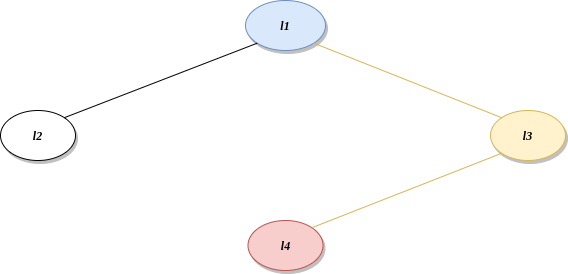
\includegraphics[scale=0.5]{figures/agent_example.png}
    \caption{Ejemplo del problema del agente. Su posición inicial es la
             ubicación $l1$ en azul queriendo llegar a la posición $l4$ marcada
             con rojo.}
    \label{fig:agent_example}
\end{figure}

\section{Representaciones STRIPS}

Un dato de entrada necesario para cualquier algoritmo de planificación es una
descripción del problema a ser resuelto. En la práctica, es usualmente imposible
incluir una enumeración explícita de todos los estados y transiciones que se
pueden realizar en el dominio a partir de una tarea STRIPS. Por lo tanto, es
necesario una representación que permita computarlas dinámicamente.

Consideremos el problema del ejemplo anterior donde se tiene el agente $a_1$
pero esta vez $n$ ubicaciones. Para este caso, se va a necesitar $n$ símbolos
proposicionales $p_i$ tal que representen la acción ``El agente $a_1$ está en la
ubicación $i$``. Si en lugar de un solo agente hubiese una cantidad $m$ de
ellos. Se necesitarían $n \times m$ símbolos para modelar esta característica de
la tarea. Una forma más compacta de representar esta propiedad es por medio de
un predicado de la forma $at(x, l)$ donde $x$ denota a un agente, y $l$ su
ubicación, siendo mucho más flexible debido a su naturaleza esquemática.

De manera similar, si se quisiera modelar una acción de cambio de posición,
haría falta describir una por cada agente y par de ubicaciones obteniendo un
total de $m \times n \times n$ instancias. Una mejor alternativa es representar
esta transformación por medio de un esquema de acción de la forma $move(x, l,
l')$ donde $x$ representa al agente, $l$ la ubicación actual, y $l'$ la
ubicación a la cual moverse.

De esta manera resulta más adecuado para la especificación utilizar predicados y
esquemas de acción en lugar de símbolos proposicionales. Esto lleva a las
siguientes definiciones:

\begin{mydef}
    Una especificación de una tarea STRIPS es una 6-upla $(\mathcal{P},
    \mathcal{A}, \Sigma^{C}, \Sigma^{O}, I, G)$  donde $\mathcal{P}$ es un
    conjunto de predicados, $\mathcal{A}$ es un conjunto de esquemas de acción,
    $\Sigma^{C}$ es un conjunto de símbolos constantes, $\Sigma^{O}$ es un
    conjunto de variables, $I \subseteq \mathcal{P}^{\Sigma^{C}}$ es el estado inicial, y
    $G \subseteq \mathcal{P}^{\Sigma^{c}}$ es la meta.

    \begin{itemize}
        \item Un esquema de acción es una 3-upla $a[X] = (pre(a), add(a),
        del(a))$ donde cada elemento es subconjunto de $\mathcal{P}$, y $X$ es
        el conjunto de variables que ocurren en $pre(a) \cup add(a) \cup del(a)$
        y que son parte de $\Sigma^{O}$.
        \item Un predicado es un símbolo atómico de $\mathcal{P}$ de la forma
        $p[X]$ con $X$ un conjunto de variables que ocurren en su interfaz y que
        son parte de $\Sigma^{O}$.
        \item $\mathcal{P}^{\Sigma^{C}}$ es el conjunto de todos los posibles
        facts que se pueden instanciar con los predicados en $\mathcal{P}$ a
        partir de los símbolos en $\Sigma^C$, es decir, el fact $\hat{p} \in
        \mathcal{P}^{\Sigma^{C}}$ si $\hat{p}$ se obtiene a partir de reemplazar
        todas las variables en $p[X]$ por objetos concretos de $\Sigma^{C}$,
        para algún $p[X] \in \mathcal{P}$.
    \end{itemize}
\end{mydef}

Para la tarea STRIPS del problema del agente una primera especificación podría
ser definida de la siguiente manera:

\begin{align*}
    \mathcal{P} = \{&at(x, l)\} \\
    \mathcal{A} = \{&move(x, l, l')\} \\
    \Sigma^{C} = \{&a_1, l_1, l_2, l_3, l_4\} \\
    \Sigma^{O} = \{&x, l, l'\} \\
    I = \{&at(a_1, l_1)\} \\
    G = \{&at(a_1, l_4)\}
\end{align*}
\begin{align*}
    move(x, l, l') &= (pre(move), add(move), del(move)) \\
                   &= (\{at(x, l)\}, \{at(x, l')\},\{at(x, l)\})
\end{align*}

Una diferencia importante es que ahora $move(x, l, l')$ es un esquema de acción
donde $x$, $l$, $l'$ son variables libres pertenecientes a $\Sigma^{O}$. De esta
manera, las variables se hicieron parte de la especificación, logrando expresar
predicados y acciones de manera esquemática.

Por otro lado, está especificación de la tarea STRIPS, instancia más acciones
que las del problema anterior, en particular, $move(a_1, l_2, l_4)$ está
especificada como un movimiento posible. Por lo tanto, para representar
exactamente el grafo de la figura \ref{fig:agent_example} es necesario agregar a
la especificación un predicado extra, $is\_connected(l, l')$, que represente la
existencia de un camino entre $l$ y $l'$. Luego, la estructura del grafo de la
figura \ref{fig:agent_example} debe incluirse en el estado inicial. Además, el
esquema de acción $move(x, l, l')$ debe poder aplicarse en un estado siempre y
cuando exista un camino entre $l$ y $l'$.

\begin{align*}
    \mathcal{P} = \{&at(x, l)\} \\
    \mathcal{A} = \{&move(x, l, l')\} \\
    \Sigma^{C} = \{&a_1, l_1, l_2, l_3, l_4\} \\
    \Sigma^{O} = \{&x, l, l'\} \\
    I = \{& at(a_1, l_1), \\
          & is\_connected(l_1, l_2), is\_connected(l_2, l_1), \\
          & is\_connected(l_1, l_3), is\_connected(l_3, l_1), \\
          & is\_connected(l_3, l_4), is\_connected(l_4, l_3)\} \\
    G = \{& at(a_1, l_4), \\
          & is\_connected(l_1, l_2), is\_connected(l_2, l_1), \\
          & is\_connected(l_1, l_3), is\_connected(l_3, l_1), \\
          & is\_connected(l_3, l_4), is\_connected(l_4, l_3)\}
\end{align*}
\begin{align*}
    move(x, l, l') &= (pre(move), add(move), del(move)) \\
                   &= (\{at(x, l), is\_connected(l, l')\}, \{at(x, l')\},\{at(x, l)\})
\end{align*}

Un detalle de esta especificación es que es no tipada. Por ejemplo $move(a_1,
a_1, a_1)$ es una acción instanciable. Lo cual deja en claro la necesidad de una
representación de tareas que preserve los tipos de los esquemas de acción y
predicados, y así evitar preprocesar acciones innecesarias durante el proceso de
grounding.

Por último, un plan que resuelve la tarea STRIPS instanciada, es a su vez un
plan para la especificación siendo está relación la que permite vincular ambas
representaciones.

\section{El lenguaje PDDL}

Para especificar una tarea de planning a una computadora se necesita definir un
lenguaje que permita al usuario definir cada una de sus componentes. Para dar
respuesta a esta necesidad surge el \emph{Planning Domain Specification
Language} (PDDL), Propuesta para la competencia de planning AIPS-98
\citep{McDermott1998} siendo el lenguaje de especificación de dominios y
problemas de planning más usado dentro de la comunidad de planning.

Una especificación en PDDL consiste de dos archivos, la definición del dominio,
donde se aclaran los predicados y esquemas de acción disponibles; y la
definición de la tarea donde se mencionan los objetos concretos a modelar, el
estado inicial, y la meta. Esta separación resulta importante, ya que diferentes
tareas de un mismo dominio comparten una estructura común. Los listing
\ref{lst:agent-domain} y \ref{lst:agent-task} muestran los archivos de dominio y
tarea del ejemplo del agente escrita en PDDL.

\begin{lstlisting}[
    float=!htb,
    caption={Dominio Agent en PDDL.},
    label={lst:agent-domain},
    language=PDDL]
  (
    define (domain AGENT-DOMAIN)

    (:requirements :strips :typing)

    (:types AGENT LOCATION)

    (:predicates (at ?x - AGENT ?l - LOCATION)
                 (is_connected ?l - LOCATION ?l' - LOCATION)
    )

    (:action move
        :parameters (?x - AGENT ?s - LOCATION ?d - LOCATION)
        :precondition (and (at ?x ?s) (is_connected ?l ?l'))
        :effect (and (not (at ?x ?s)) (at ?x ?d))
    )
  )
\end{lstlisting}

\begin{lstlisting}[
    float=!htb,
    caption={Ejemplo de una tarea del dominio Agent en PDDL.},
    label={lst:agent-task},
    language=PDDL]

  (
    define (problem AGENT-TASK)

    (:domain AGENT-DOMAIN)

    (:objects a1 - AGENT l1 l2 l3 l4 - LOCATION)

    (:init at(a1, l1)
           (is_connected l1 l2)
           (is_connected l2 l1)
           (is_connected l1 l3)
           (is_connected l3 l1)
           (is_connected l3 l4)
           (is_connected l4 l3)
           (is_connected l1 l2)
           (is_connected l2 l1)
           (is_connected l1 l3)
           (is_connected l3 l1)
           (is_connected l3 l4)
           (is_connected l4 l3)
    )
    
    (:goal (and 
           (at a1 l4)
           (is_connected l1 l2)
           (is_connected l2 l1)
           (is_connected l1 l3)
           (is_connected l3 l1)
           (is_connected l3 l4)
           (is_connected l4 l3)
           (is_connected l1 l2)
           (is_connected l2 l1)
           (is_connected l1 l3)
           (is_connected l3 l1)
           (is_connected l3 l4)
           (is_connected l4 l3)
           )
    )
  )
\end{lstlisting}

Observar que tanto los predicados como las acciones están parametrizados con
variables de un cierto tipo. Por ejemplo para el predicato $at(x, y)$, $x$ es de
tipo \emph{AGENT} e $y$ del tipo \emph{LOCATION} ambos previamente listados en
la línea 6 del listing \ref{lst:agent-domain}. Luego en la línea 7 del listing
\ref{lst:agent-task} se especifican todos los objetos disponibles y el tipo al
cual corresponden.

\section{Relajación por deletes}
\label{lit:delete_relaxed}

El problema de decidir si una tarea de planning STRIPS tiene un plan es
PSPACE-completo. Es por eso que las implementaciones que lo resuelven son a
partir de algoritmos de búsqueda de orden exponencial. El planificador instancia
un problema y realiza una búsqueda exhaustiva guiada por medio de una función
heurística definida a partir de \emph{planes relajados}. Un plan relajado es un
plan en un dominio donde a todas las acciones se les eliminaron los efectos
negativos. Es decir su lista $del$. Si bien no es exactamente el dominio sobre
el cual se desea resolver la tarea original, brinda información relevante para
hallar una solución. En particular, si los planes relajados permiten guiar la
búsqueda para encontrar un plan de la tarea, entonces también podría ser usado
para guiar el proceso de grounding.

Los planes relajados son secuencias de acciones cuyos efectos negativos son
eliminados, son aplicables en el estado inicial, y su estado resultante contiene
a la meta. Esto proviene de la \emph{relajación por deletes}, una simplificación
de la tarea de planning que consiste en eliminar los efectos negativos de las
acciones. Esta relajación es ampliamente utilizada en planning y su importancia
subyace en la siguiente propiedad: en la \emph{relajación por deletes} si un
\emph{fact} $p$ se vuelve verdadero en un estado $s$, entonces para toda
secuencia de acciones $\vec{a} \in A^{*}$ aplicables en $s$, el estado
resultante también hará verdadero $p$. Por ejemplo, en el problema del agente,
si este se desplazó por varias ubicaciones, tendríamos que se encuentra en más
de un lugar al mismo tiempo, ya que la proposición que indicaba su ubicación
anterior no puede ser borrada. Esta propiedad es la que permite que computar un
plan en el dominio relajado sea polinomial en comparación al dominio original.

\begin{mydef}
    Sea $\Pi = (F, A, I, G)$ una tarea STRIPS.
    \begin{itemize}
        \item Sea $a \in A$, definimos a la acción relajada por delete $a^{+}$
        dada por $pre(a^{+}) = pre(a)$, $add(a^{+}) = add(a)$, y $del(a^{+}) =
        \emptyset$.

        \item Denotaremos con $A^{+} = \{a^{+} : a \in A\}$ al conjunto de
        acciones relajadas por delete.

        \item Para una secuencia de acciónes $\vec{a}$ denotaremos con
        $\vec{a}^{+}$ a la secuencia de acciones relajadas por delete.

        \item Denotaremos con $\Pi^{+} = (F, A^{+}, I, G)$ a la tarea STRIPS
        relajada por deletes.

        \item Un plan relajado para $\Pi$ es un plan para $\Pi^{+}$.
    \end{itemize}
\end{mydef}

Claramente es una modelización no realista, no obstante, relajar una tarea
STRIPS provee información importante sobre la tarea original, en particular:

\begin{lemma}
\label{lit:delete_relaxed_property}
Sea $\Pi = (F, A, I, G)$ Una tarea STRIPS
\begin{itemize}
    \item Si una secuencia de acciones $\vec{a}$ es un plan de $\Pi$, entonces
    $\vec{a}^{+}$ es un plan relajado de $\Pi$.
    \item Si no existe un plan para $\Pi^{+}$ entonces no existe un plan para
    $\Pi$.
\end{itemize}
\end{lemma}

Estas propiedades serán muy relevantes al introducir los algoritmos de grounding
en las secciones \ref{lit:relaxed_grounding}, y \ref{lit:heuristic_grounding}.
La primera de ellas nos dice que un plan de una tarea STRIPS, es a la vez un
plan de la tarea relajada. No obstante el recíproco no se cumple. Por lo
general, un plan en la tarea relajada no es un plan de la tarea original. La
segunda de ellas menciona que si no existe un plan para la tarea relajada,
entonces no hay un plan para la tarea original. Esto también es importante, ya
que todo plan en la tarea relajada puede encontrarse con solo instanciar
aquellas acciones que sean alcanzables. Si no se encuentra un plan de la tarea
relajada para ese conjunto de acciones, entonces sabremos que no existirá
solución en la tarea original.

\section{Proceso de grounding}
\label{lit:relaxed_grounding}

Dada una especificación de una tarea STRIPS $(\mathcal{P}, \mathcal{A},
\Sigma^{C}, \Sigma^{O}, I, G)$ se puede obtener su correspondiente tarea $\Pi =
(F, A, I, G)$ recolectando todas las instancias posibles de predicados en
$\mathcal{P}$ y esquemas de acción de $\mathcal{A}$ con objetos de $\Sigma^{C}$.
Es decir, $F$ contiene un \emph{fact} por cada posible asignación de objetos a
los argumentos de cada predicado $P[X] \in \mathcal{P}$, y $A$ contiene una
acción por cada posible asignación de objetos a los argumentos de cada esquema
de acción $a[X] \in \mathcal{A}$. Este proceso se conoce como \emph{grounding
cartesiano}.

No obstante, en la práctica los planificadores no instancian todas las posibles
acciones y proposiciones, sino aquellas que son alcanzables relajadamente desde
el estado inicial debido al lemma \ref{lit:delete_relaxed_property}.

Este proceso de grounding es el implementado por \emph{Fast Downward}
\citep{Helmert-2011}, el sistema de planning clásico basado en búsqueda
heurística más popular por la comunidad debido a su excelente desempeño en
benchmarks, competencias internacionales de planning, e implementaciones
eficientes de algoritmos genéricos de búsqueda. Estas implementaciones son
altamente configurables por Fast Downward permitiendo ajustarse a distintos
dominios de planning. Su popularidad y versatilidad fue la motivación que nos
llevó a utilizarlo en esta tesis en comparación a otros sistemas.

\begin{mydef}
    Sea $\Pi = (F, A, I, G)$ una tarea STRIPS.    
    \begin{itemize}
        \item Un estado $s \subseteq F$ es alcanzable en $\Pi$ si existe una
        secuencia $\vec{a} \in A^{*}$ tal que $I \xrightarrow{\vec{a}} s$.
    
        \item Una proposición $p \in F$ es alcanzable en $\Pi$ si existe un
        estado $s$ alcanzable en $\Pi$ tal que $p \in s$.

        \item Una acción $a \in A$ es alcanzable en $\Pi$ si existe un estado
        $s$ alcanzable en $\Pi$ tal que $a$ es aplicable en $s$.

        \item Una proposición $p \in F$ es alcanzable relajadamente en $\Pi$ si
        $p$ es alcanzable en $\Pi^{+}$.

        \item Una acción $a \in A$ es alcanzable relajadamente en $\Pi$ si
        $a^{+}$ es alcanzable en $\Pi^{+}$.
    \end{itemize}
\end{mydef}


\begin{algorithm}
    \caption{Grounding por alcanzabilidad
    relajada}\label{alg:grounding_delete_relaxed}
    \begin{algorithmic}[1]
    \Require Especificación de una tarea STRIPS $(\mathcal{P}, \mathcal{A},
    \Sigma^{C}, \Sigma^{O}, I, G)$ \Ensure Tarea STRIPS $(F, A, I, G)$ \State $q
    \gets Queue(I)$ \State $F \gets \emptyset$ \State $A \gets \emptyset$
    \While{$ \lnot q.empty()$} \State $e \gets q.pop()$ \If{$e.isFact()$} \State
    $F \gets F \cup \{e\}$ \For{$a \notin A \land pre(a) \subseteq F$} \State
    $q.insert(a)$ \EndFor \Else \State $A \gets A \cup \{e\}$ \For{$f \notin F
    \land f \in add(e)$} \State $q.insert(f)$ \EndFor \EndIf \EndWhile \State
    \Return $(F, A, I, G)$
    \end{algorithmic}
\end{algorithm}

El algoritmo \ref{alg:grounding_delete_relaxed} implementado por Fast Downward
parte de una cola $q$ que almacena todos los símbolos proposicionales del estado
inicial. Luego la cola $q$ almacena elementos a preprocesar que pueden ser tanto
facts como acciones. A partir de allí, se remueve elemento a elemento de $q$
consultando si es un fact o una acción.

En el caso de encontrarse con un fact, se lo instancia y se agregan a $q$ todas
las acciones aplicables (aún no procesadas) a partir de las proposiciones
groundeadas hasta el momento. Caso contrario, se obtiene una acción que también
se instancia y se agregan a $q$ todas las proposiciones (aún no procesadas) que
ocurren positivamente en su efecto, es decir, su lista $add$.

Este procedimiento se repite hasta que la cola se encuentre vacía, obteniendo de
esta manera todas las acciones y facts alcanzables relajadamente.

\section{Grounding heurístico}
\label{lit:heuristic_grounding}

Mencionamos que un plan de una tarea es también un plan relajado de la misma.
Sin embargo, el recíproco no se cumple. Es más, un hecho o una acción que es
relajadamente alcanzable, puede no ser alcanzable en la tarea original o ser
irrelevante al no pertenecer a ningún plan que la resuelva. Es justamente esta
pérdida de información la que origina que computar en el mundo relajado sea
polinomial. Es aquí donde surge el foco de este trabajo donde se intentará
predecir cuál de estos hechos y acciones son verdaderamente relevantes para
alcanzar la meta, priorizando su instanciación por sobre el resto.

\begin{algorithm}
    \caption{Grounding heurístico}\label{alg:grounding-heuristico}
    \begin{algorithmic}[1]
    \Require Especificación de una tarea STRIPS $(\mathcal{P}, \mathcal{A},
    \Sigma^{C}, \Sigma^{O}, I, G)$. Número máximo de instanciaciones permitidas
    $N$ \Ensure Tarea STRIPS $(F, A, I, G)$ \State $q \gets PriorityQueue(I)$
    \State $F \gets \emptyset$ \State $A \gets \emptyset$ \While{$ \lnot
    (q.empty() \lor G \subseteq F) \land |A| \leq N$}    
    \If{$q.containsFact()$} \State $f \gets q.popFact()$ \State $F \gets F \cup
        \{f\}$ \For{$a \notin A \land pre(a) \subseteq F$} \State $q.insert(a)$
        \EndFor \Else \State $a \gets q.popHighPriorityAction()$ \State $A \gets
        A \cup \{a\}$ \For{$f \notin F \land f \in add(a)$} \State $q.insert(f)$
        \EndFor \EndIf \EndWhile \State \Return $(F, A, I, G)$
    \end{algorithmic}
\end{algorithm}

El algoritmo de grounding heurístico que presentaremos es el mismo que se
desarrolló en \citep{Gnad_Torralba_Dominguez_Areces_Bustos_2019} y está basado
en el que se mostró en la sección anterior. Las principales diferencias son el
criterio de parada, donde se procesan no más de $N$ acciones, y el orden en que
lo hacen, según su nivel de relevancia. Debido a que el algoritmo puede terminar
antes de que la cola se vacíe, se está obligado a procesar la totalidad de los
facts existentes en la cola antes de considerar una siguiente acción. Esto
garantiza que todos los facts que se encuentran en los efectos de las acciones
ya procesadas están en $F$, siendo el algoritmo \emph{fact consistente}.

\begin{mydef}
    Sean $F$ y $A$ el conjunto de facts y acciones retornadas por un algoritmo
    de grounding. Decimos que este es fact consistente si para todo $a \in A$ se
    cumple que, si $p \in pre(a) \cup add(a) \cup del(a)$ entonces $p \in F$.
\end{mydef}

En grounding heurístico, el algoritmo puede detenerse mucho antes según el
parámetro $N$ que indica la cantidad de instancias que puede realizar el proceso
sin que los recursos de tiempo y memoria se vean comprometidos. Por lo general,
muchas de los problemas de planning requieren planes cortos del orden de a lo
sumo cientos de acciones en comparación a posiblemente millones de operadores
groundeados.

Es importante mencionar que este algoritmo es \emph{correcto}, si hallamos un
plan de la tarea obtenida por grounding heurístico, entonces ese mismo plan lo
es para la tarea obtenida por grounding total. No obstante, no es
\emph{completo}, una tarea obtenida por grounding heurístico tiene solución si y
sólo si las acciones correspondientes de al menos un plan (de la tarea obtenida
por grounding total) fueron procesadas.

Por último, algo a considerar es el remplazo de la cola del Algoritmo
\ref{alg:grounding-heuristico}, por una cola de prioridades que asigna a las
acciones un nivel de relevancia por la cual son ordenadas. La relevancia de una
acción está directamente relacionada con la probabilidad de que esta pertenezca
a un plan de la tarea. Notar que una estimación ideal sería una probabilidad de
1 para las acciones que ocurren en algún plan de la tarea y 0 para las
restantes. Pero computar esto es tan difı́cil como obtener una solución y
sabemos que es PSPACE-completo. Es por eso que para estimar la relevancia se
utilizaron técnicas de aprendizaje automático y serán el foco del siguiente
capítulo.
